% WACV 2027 Paper Template
% Converted manuscript project

\documentclass[10pt,twocolumn,letterpaper]{article}

\usepackage[datasets]{wacv}

% Additional packages for the converted manuscript.
\usepackage{times}
\usepackage{epsfig}
\usepackage{graphicx}
\usepackage{amsmath}
\usepackage{amssymb}
\usepackage{booktabs}
\usepackage{threeparttable}
\usepackage{tabularx}
\usepackage{array}
\usepackage{multirow}
\usepackage{makecell}
\usepackage{adjustbox}
\usepackage{tikz}
\usetikzlibrary{arrows.meta,positioning}
\usepackage{float}
\usepackage{enumitem}
\usepackage{xspace}
\usepackage{xurl}
\usepackage{microtype}

\providecommand{\ie}{i.e.\xspace}
\providecommand{\eg}{e.g.\xspace}
\providecommand{\etal}{et al.\xspace}
\newcommand{\kappascore}{\ensuremath{\kappa}\xspace}
\newcommand{\mf}{macro-F1\xspace}
\newcommand{\PATHOGAIT}{\textsc{PathoGait}\xspace}
\newcommand{\ATAXIA}{\textsc{Ataxia}\xspace}
\newcommand{\GMFCS}{\textsc{GMFCS}\xspace}
\newcommand{\PARKINSONISM}{\textsc{Parkinsonism}\xspace}
\newcommand{\red}[1]{{\color{red}#1}}
\newcommand{\todo}[1]{{\color{red}#1}}
\newcommand{\TODO}[1]{\textbf{\color{red}[TODO: #1]}}


\definecolor{wacvblue}{rgb}{0.21,0.49,0.74}
\usepackage{xr} % [Fan R2 A2] resolve \ref{...supp...} against the separate supplement build
% Cross-document labels are not needed by this self-contained main draft.
\usepackage[pagebackref,breaklinks,colorlinks,allcolors=wacvblue]{hyperref}

\def\wacvPaperID{*****}
\def\confName{WACV}
\def\confYear{2027}

\title{GaitEval: A Multi-Condition Benchmark for Evaluating Whether Large Language Models Use Pose-Derived Gait Evidence}

\author{Author names, order, affiliations, and emails pending verification\\
Submission 01586 --- author metadata to be completed before upload}

\begin{document}
\maketitle

\begin{abstract}
Pose-based gait data are widely used for clinical screening, yet whether Large Language Models (LLMs) can interpret such motion evidence remains underexplored.
We introduce GaitEval, a six-dataset benchmark for evidence-grounded label prediction across ASD-Kinect, ATAXIA, CARE-PD, GMFCS, PARKINSONISM, and PATHOGAIT, with heterogeneous populations, pose formats, and label spaces.
A baseline-anchored protocol compares controlled pose-derived inputs with label-prior and same-feature linear references, and evaluates zero-shot, few-shot, and low-rank adaptation (LoRA) within their tested coverage.
The retained five-family motion-summary evaluation shows near-chance agreement on its original tasks; a shared six-dataset, subject-disjoint Qwen2.5-7B evaluation identifies important dataset--representation exceptions.
Linear references recover task-relevant signal where available, while adaptation recovers some in-distribution mappings: standardized GMFCS summary macro-F1 rises from 0.265 to 0.467, but remains below its matched linear reference of 0.579.
The accepted-protocol ATAXIA result likewise retains its agreement increase from $\kappa=0.046$ to $0.507$; transfer remains unreliable in the tested bidirectional ATAXIA--PATHOGAIT probe.
Overall, evidence use is heterogeneous and representation-dependent: adaptation can learn dataset-specific mappings, while reliability beyond the tested settings remains unresolved.
\end{abstract}


\begin{figure*}[t]
\centering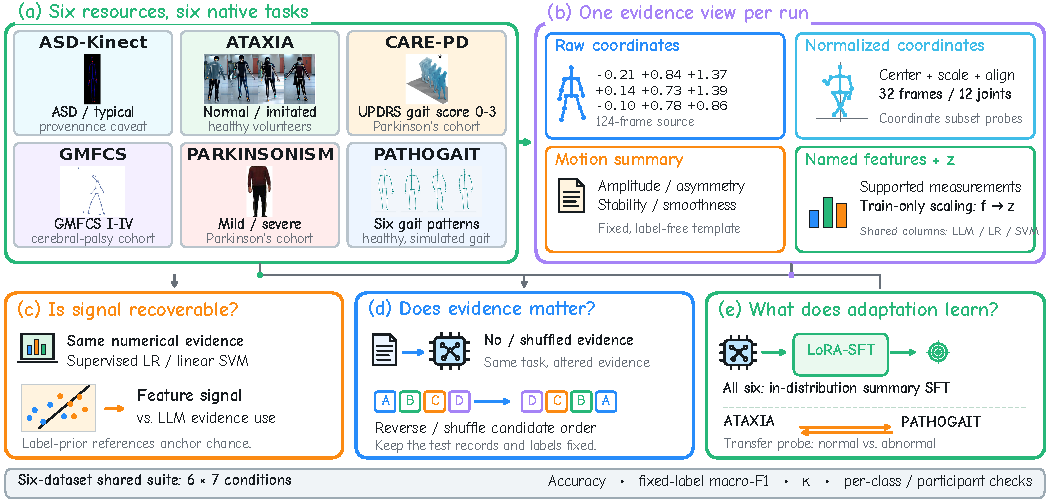
\includegraphics[width=\textwidth]{figures/overview.pdf}
\caption{\textbf{GaitEval overview.} Six datasets enter one evidence-grounded benchmark. Source-publication examples and recorded-skeleton renderings illustrate the resources; they are not matched test cases or inputs to an image model. One pose-derived evidence view is supplied per run. Same-feature references test recoverable signal; evidence/order controls, adaptation, and scoped transfer test the limits of LLM use. Source attribution and experiment coverage are documented in the supplement.}
\label{fig:method_pipeline}
\end{figure*}

\section{Introduction}

Human gait provides an accessible signal for assessing balance, coordination, strength, and mobility~\cite{perry1992gait,baker2006gait,muro2014gait}. Advances in video-based pose estimation allow ordinary walking videos to be converted into skeleton trajectories without specialized motion-capture systems~\cite{cao2017openpose,lugaresi2019mediapipe,bazarevsky2020blazepose}. Clinical reviews describe how this low-cost route has been used across neurological and rehabilitation settings~\cite{stenum2021applications,stenum2024clinical}. Pose trajectories provide a compact, anatomically indexed representation from which interpretable measurements of motion, symmetry, stability, and variability can be derived~\cite{winter2009biomechanics,schwartz2008gdi}.

Most pose-based clinical gait methods are task-specific supervised systems that map skeleton sequences to gait classes, severity levels, or clinical scores~\cite{khalil2022ataxia,deng2024parkinsonism}. Clinical studies have related quantitative gait measurements to motor severity and function in cerebral palsy, Parkinsonian impairment, and ataxia~\cite{kidzinski2020video,lu2020updrs,khalil2022ataxia}. Related visual studies span heterogeneous cohorts, acquisition settings, and label definitions~\cite{jun2020pathological,deng2024parkinsonism,khalil2022ataxia}, complicating direct cross-resource comparisons. Thus, cross-condition evaluation is not itself the novelty of this work. Instead, we ask whether LLM predictions are grounded in supplied pose-derived evidence. This distinction is important because many gait resources contain numerous clips from relatively few participants, requiring participant-aware interpretation.

Pose evidence can be presented as raw coordinates, deterministic motion summaries, or biomechanical features. Poor performance may therefore reflect limited task-relevant signal, difficulty interpreting the representation, or failure to map informative evidence to dataset-specific labels. Accuracy alone cannot distinguish these cases, particularly for imbalanced ordinal and multi-class tasks~\cite{opitz2019macro,sokolova2009performance}. Evaluation should therefore compare LLMs with label-prior baselines and simple classifiers trained on the same evidence.

We introduce \textbf{GaitEval}, a multi-condition benchmark in which \emph{gait reasoning} means grounding dataset-specified label predictions in pose-derived evidence, rather than open-ended diagnosis or clinical interpretation. The benchmark comprises six datasets: ASD-Kinect, ATAXIA, CARE-PD, GMFCS, PARKINSONISM, and PATHOGAIT. Each retains its population provenance and native label space. GaitEval introduces no new clinical recordings; it provides controlled representations, evidence-use tests, and same-feature diagnostic references (Fig.~\ref{fig:method_pipeline}).

The evaluation follows the original evidence ladder: zero-shot prompting, few-shot examples, and LoRA adaptation, with transfer limited to the tested ATAXIA--PATHOGAIT pair~\cite{brown2020fewshot,hu2022lora}. The common six-dataset analysis uses Qwen2.5-7B-Instruct, subject-disjoint partitions, and capture-quality-free features. Additional model, view, and adaptation measurements retain their original protocol labels and are never substituted for missing common-protocol experiments.

Our main contributions are:
\begin{itemize}[leftmargin=*,nosep]
\item We introduce GaitEval, a six-dataset benchmark for testing whether LLM predictions are grounded in pose-derived gait evidence across heterogeneous resources, representations, and label spaces.
\item We provide a baseline-anchored protocol that separates limited input signal from failed evidence use by comparing controlled LLM inputs with label-prior and linear feature-based references.
\item We evaluate an evidence ladder from zero-shot prompting to few-shot adaptation and LoRA fine-tuning within its measured coverage, showing in-distribution recovery on selected tasks but no reliable transfer on the tested compatible dataset pair.
\end{itemize}

\section{Related Work}

\subsection{Clinical Gait Analysis and Pose-Based Representations}

Clinical gait analysis supports assessment of motor impairment, functional severity, and rehabilitation outcomes~\cite{perry1992gait,baker2006gait,simon2004gait}. Video-based pose estimation offers an accessible alternative to laboratory motion capture by converting ordinary recordings into joint trajectories~\cite{stenum2021applications,stenum2024clinical}. Markerless toolkits and smartphone-based pipelines further broaden access to quantitative movement analysis~\cite{mathis2018deeplabcut,uhlrich2023opencap}. Validation studies have compared video-derived temporal and kinematic measures with instrumented walkways or motion-capture systems across different gait patterns and clinical cohorts~\cite{verlekar2019validation,yamamoto2021openpose,sabo2022validity}. These studies also show that viewpoint, occlusion, pose-estimation error, and population differences remain important sources of measurement uncertainty.

Gait resources differ in population, acquisition setup, skeleton format, and label definition~\cite{kidzinski2020video,khalil2022ataxia,jun2020pathological}. Pose data provide a shared semantic interface, but do not make these resources clinically equivalent. GaitEval therefore preserves each resource's native representation and dataset-defined task.

\subsection{Visual and Pose-Based Pathological Gait Analysis}

Pose-based gait systems use biomechanical features or learned temporal representations for supervised prediction. Graph models such as ST-GCN, 2s-AGCN, and MS-G3D are widely used for skeleton analysis~\cite{yan2018stgcn,shi2019twostream,liu2020disentangling}, but are generally tied to fixed datasets, skeletons, and label spaces.

Early low-cost RGB and RGB-D systems measured or classified pathological gait using semantic gait features, silhouettes, or tracked skeletons~\cite{dolatabadi2017pathological,verlekar2018automatic,ortells2018vision}. Parkinsonian assessment has since ranged from single-camera kinematic measurement and natural-gait monitoring to learned skeleton--silhouette models for clinical severity estimation~\cite{shin2021quantitative,sabo2020parkinsonian,zeng2023video}. Related work has also estimated cerebral-palsy gait function and kinematics and quantified gait after stroke from ordinary videos~\cite{kidzinski2020video,pantzar2018cerebral,lonini2022stroke}.

For ataxia, Auto-Gait analyzes clinically recorded gait-task videos from multiple sites, while pose-based work has also evaluated performed ataxic gait~\cite{rahman2023autogait,khalil2022ataxia}. A separate clinical study used video keypoints to distinguish Parkinson's disease from spinocerebellar degeneration, showing that cross-condition visual analysis predates GaitEval~\cite{eguchi2024differentiating}. Broader abnormal-gait resources include simulated pathological patterns and clinically annotated abnormal-gait videos~\cite{jun2020pathological,ranjan2024gavd}. Collectively, these studies establish that visual and pose features can support condition-specific prediction; results from performed or simulated gait, however, do not establish patient-level diagnostic validity.

Cross-dataset gait analysis is also established. Transfer-learning and spatiotemporal classifiers have been evaluated across separately collected pathological-gait datasets~\cite{verlekar2018transfer,albuquerque2021spatiotemporal}. Auto-Gait includes leave-one-site-out evaluation, and CARE-PD formalizes within-dataset, cross-dataset, leave-one-dataset-out, and adaptation protocols~\cite{rahman2023autogait,adeli2025carepd}. GaitEval therefore does not claim domain-shift difficulty as a new finding. Instead, it tests whether general-purpose LLMs use supplied pose evidence under same-input controls. Logistic regression and a linear support vector machine receive the same deterministic features, and the ATAXIA--PATHOGAIT transfer experiment is limited to that compatible dataset pair.

\subsection{Language Models for Human Motion and Clinical Gait}

Motion-language systems such as MotionGPT, MotionLLM, and MoChat connect language models with motion through learned tokenization or cross-modal alignment~\cite{jiang2023motiongpt,chen2024motionllm,mo2024mochat}. Gait-specific models have also been developed for biometric recognition and Parkinsonian scoring~\cite{yang2025gaitllm,wang2025agir}. BiomechGPT and BioGait-VLM further connect language-aligned representations with clinically relevant movement analysis~\cite{yang2025biomechgpt,chen2026biogait}. These methods rely on task-specific motion-language training rather than testing off-the-shelf LLM evidence use.

The closest concurrent work evaluates general-purpose LLMs using text-encoded kinematic waveforms~\cite{dindorf2026gaitllm}. More broadly, prior work has examined LLMs for structured and tabular inputs~\cite{fang2024llms} and multimodal instruction following~\cite{liu2023llava,yin2024survey}. GaitEval instead evaluates heterogeneous gait resources through controlled pose-derived views, same-feature linear references, and adaptation experiments. Its purpose is to separate limited motion signal from representation difficulty and failed LLM evidence use, while restricting transfer conclusions to the tested dataset pair.

\section{Methods}
\label{sec:methods}
\subsection{Source Sequences and Dataset Tasks}
\label{sec:benchmark_formulation}
GaitEval evaluates dataset-specified label prediction from pose-derived evidence. The six datasets and their evaluation partitions are listed in Table~\ref{tab:method_datasets}. GMFCS contains children with cerebral palsy~\cite{palisano1997gmfcs}; PARKINSONISM and CARE-PD concern Parkinson's disease with different severity or gait-item targets~\cite{deng2024parkinsonism,adeli2025carepd}. ATAXIA contains healthy volunteers imitating ataxic gait~\cite{khalil2023dataset}, and PATHOGAIT contains healthy volunteers simulating six gait patterns~\cite{jun2020pathological}. ASD-Kinect defines an autism-versus-typical task~\cite{aljubouri2021asd}; its source reports some movements simulated by others without identifying the affected sequences. These resources are therefore not six interchangeable clinical cohorts.

\begin{table*}[t]
\centering\small
\caption{\textbf{Six benchmark datasets for the seven-condition evaluation (source-reported subject-disjoint partitions).} Counts are eligible train/test clips and test participants, not full-source cohort sizes. All six datasets have summary and z-feature zero-shot, evidence/order controls, summary-SFT, and matched LR/SVM.}
\label{tab:method_datasets}
\begin{tabular*}{\textwidth}{@{\extracolsep{\fill}}lllrr@{}}\toprule
Dataset & Population & Task & Train / test & Test subjects\\\midrule
ASD-Kinect & ASD / typical; provenance caveat & Binary & 70 / 20 & 20\\
ATAXIA & Healthy, imitated gait & Binary & 28 / 8 & 4\\
CARE-PD & Multi-site Parkinson's cohort & UPDRS gait 0--3 & 1901 / 665 & 24\\
GMFCS & Cerebral-palsy cohort & Four-level ordinal & 914 / 255 & 149\\
PARKINSONISM & Parkinson's cohort & Binary severity & 83 / 29 & 5\\
PATHOGAIT & Healthy, simulated gait & Six patterns & 5040 / 1440 & 2\\\bottomrule
\end{tabular*}
\end{table*}

A source sequence is $X_i\in\mathbb{R}^{T_i\times J_d\times C_d}$, with dataset-specific joints and coordinate channels. Native 2D/3D representations follow established pose formats~\cite{cao2017openpose,ionescu2014human36m}. GaitEval applies one evaluation protocol: select task-eligible participant partitions; derive a label-redacted input view; run the declared model and evidence condition; fit supervised transformations on training data only; and score predictions against the complete task label set. Each experiment records its model, input construction, test IDs, and parser settings. The coordinate-input experiments use a 124-frame source tensor, with padding masked during feature computation; normalized-coordinate prompts sample 32 frames and 12 common joints. Feature and summary runs aggregate the valid trajectories in their recorded input construction.

All six datasets enter the seven-condition Qwen2.5-7B evaluation on the test sets in Table~\ref{tab:method_datasets}. Additional model, coordinate, few-shot, and feature-SFT experiments use the eligible records listed in the supplemental evaluation-record inventory; their test counts are also stated with the results. The GMFCS split-repair check uses 866 test clips from 166 participants; the seven-condition comparison uses 255 clips from 149 participants. Within an experiment, comparisons use matched test records; comparisons across different test populations are descriptive. Participant separation in the 866-clip experiment is independently verified. The seven-condition partitions are reported as subject-disjoint by the source metadata, but complete training manifests remain unavailable for an independent check. Section~\ref{sec:review_checks} documents the repair.

\subsection{Controlled Input Views}
\label{sec:input_views}
Each run exposes one view. Four input-view families are defined: raw coordinates, normalized coordinates, deterministic motion summaries, and named biomechanical features. A train-statistics z-scored encoding is a scaling control within the feature family, not a fifth modality. Coordinate prompting is a subset experiment; it is not claimed to have common six-dataset coverage.

Features describe motion range, bilateral asymmetry, trunk/pelvis variability, trajectory variance, and jerk-based smoothness~\cite{winter2009biomechanics,schwartz2008gdi}. Unsupported joints are omitted consistently from the LLM and matched linear inputs. These are pose-coordinate descriptors, not calibrated physical stride lengths or forces. The jerk descriptor uses third finite differences per frame and is not asserted to have SI jerk units. For feature $f$, scaling is $z=(f-\mu_{\rm tr})/\sigma_{\rm tr}$, using training statistics only; constant and missing-column handling is specified in the supplement.

Motion summaries are generated by a deterministic, label-independent template from the numerical measurements, not by annotators, dataset metadata, or another LLM. They preserve numbers and fixed qualitative descriptors. Capture-quality variables, including valid-frame fraction, are excluded from the seven shared feature/summary conditions. Model-visible inputs exclude answer-revealing labels, dataset names, participant IDs, demographics, and clinical metadata; candidate labels remain because they define the task. Figure~\ref{fig:method_detail} distinguishes these transformations.

\begin{figure}[t]
\centering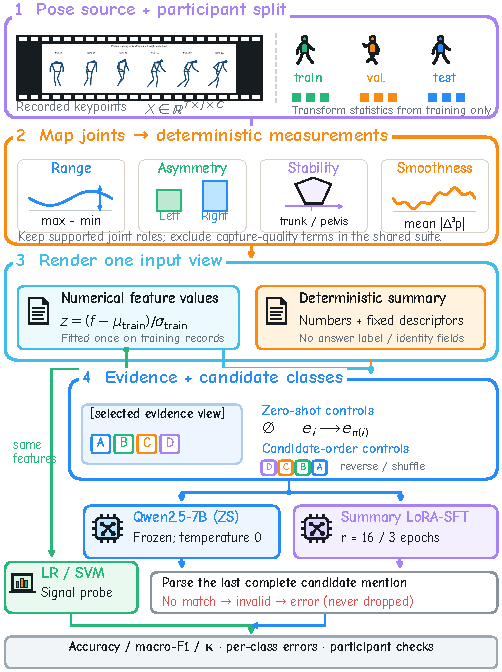
\includegraphics[width=\columnwidth]{figures/methods.pdf}
\caption{\textbf{Pose-to-label evaluation.} The shared six-dataset workflow links training-only transformations to zero-shot controls, summary-SFT, and matched linear references. Recorded GMFCS keyframes illustrate the source; measurement glyphs are schematic. Invalid outputs remain errors. Optional probes follow the supplemental coverage.}
\label{fig:method_detail}
\end{figure}

\subsection{Models, Adaptation, and Evidence Controls}
\label{sec:evaluation_settings}
The five-family motion-summary axis evaluates Llama-3.3-70B, Qwen2.5-72B, and Gemma-3-27B~\cite{grattafiori2024llama3,qwen2024qwen25,gemma2025gemma3}, together with GLM-4-32B and DeepSeek-R1-Distill-Qwen-32B~\cite{glm2024chatglm,guo2025deepseekr1}. The shared six-dataset axis fixes Qwen2.5-7B-Instruct. The test counts for the five-model comparison are 20, 1,647, 665, 866, 120, and 2,181 clips in dataset order; the corresponding Qwen-7B shared-condition counts are in Table~\ref{tab:method_datasets}. Full settings and coverage are in the supplement.

All six datasets use seven common conditions: summary zero-shot; z-feature zero-shot; no evidence; shuffled evidence; reversed and shuffled candidate order; and summary LoRA-SFT. Shuffled evidence deranges summaries across test records while preserving candidate labels. Candidate-order controls preserve evidence and change only label presentation. Decoding is deterministic. The parser chooses the last complete, boundary-anchored candidate mention, resolving same-position matches by length. It does not validate the model's reasoning. Outputs with no matching candidate count as errors.

Few-shot prompting prepends fixed class-balanced training examples~\cite{brown2020fewshot}. The tested settings are 8/16/32 examples on ATAXIA, 16 on PARKINSONISM, and 12 on PATHOGAIT; other cells are unexecuted. A reasoning-anchored summary prompt asks for salient motion evidence and candidate comparison~\cite{wei2022cot}; it is also a scoped probe.

LoRA adapts Qwen2.5-7B separately per dataset~\cite{hu2022lora}. The summary-SFT recipe for the seven shared conditions uses rank 16, $\alpha=32$, dropout 0.05, all linear projections, completion-only loss, three epochs, learning rate $10^{-4}$, and effective batch size 16. It saves the final adapter without validation checkpoint selection. No new training is claimed in this revision. Complete prompts, experiment-specific settings, inference budgets, and configuration coverage are given in the supplement.

\subsection{References, Metrics, and Scope}
\label{sec:metrics}
Label-prior predictors and class-balanced logistic regression (LR) and linear SVM~\cite{cortes1995svm,pedregosa2011scikit} anchor interpretation. LR/SVM receive the exact deterministic feature columns underlying the corresponding LLM feature view; they are supervised signal probes, not zero-shot competitors or clinical state of the art.

Accuracy, fixed-label-set macro-F1, and Cohen's $\kappa$~\cite{cohen1968weighted,opitz2019macro,sokolova2009performance} are reported jointly. Here $\kappa=(p_o-p_e)/(1-p_e)$, with $p_e$ obtained from the empirical target and prediction marginals. Invalid responses remain errors. Ordinal tasks additionally report quadratic-weighted $\kappa$ and absolute level error. Macro-F1 uses the complete task label set even when a class is unpredicted.

Participant-cluster bootstrap resampling uses 2,000 draws~\cite{efron1993bootstrap}. Historical bootstrap intervals and paired tail areas are identified separately from fixed-label point metrics, since absent classes and an invalid-output sentinel can change the resampled label set. Very small participant counts limit inference regardless of the number of clips. PATHOGAIT's two-participant results are descriptive; no participant-population superiority is claimed. Multiple exploratory contrasts are reported without a family-wide significance claim.

Transfer is measured only on the ATAXIA--PATHOGAIT pair after harmonizing normal versus abnormal gait. A model adapted on one dataset is tested on the other without target labeled examples. This probes combined condition and representation shift; no transfer result is claimed for unmatched severity, gait-score, or ASD targets.

\section{Experiments}
\label{sec:experiments}
\subsection{Shared Six-Dataset Evaluation}
The shared S evaluation fixes the same model, input derivation contract, controls, and eligible test records within each dataset. Table~\ref{tab:shared_results} reports all six datasets together. The 42 common cells are backed by individual predictions; two extra raw-feature cells and ten five-family cells provide incomplete additional axes. One archived mixed-task CARE-PD diagnostic is excluded from the common task. No unexecuted cell is interpreted as a failure.

\begin{table*}[t]
\centering\small
\caption{\textbf{Same-model evidence use and adaptation across all six datasets (S).} Values are macro-F1, recomputed from released predictions with a fixed task label set. LR/SVM values are the committed task-matched supervised references. $N$ is clips/participants. Best LLM view is bold; bold does not imply superiority over references.}
\label{tab:shared_results}
\begin{tabular*}{\textwidth}{@{\extracolsep{\fill}}lrrrrrrr@{}}\toprule
Dataset & $N$ & Chance & ZS summary & ZS z-features & Summary SFT & LR & SVM\\\midrule
ASD-Kinect & 20/20 & .490 & .310 & \textbf{.436} & .310 & .697 & .744\\
ATAXIA & 8/4 & .488 & .273 & \textbf{.333} & \textbf{.333} & .873 & .873\\
CARE-PD & 665/24 & .250 & .321 & .133 & \textbf{.445} & .659 & .650\\
GMFCS & 255/149 & .250 & .265 & .150 & \textbf{.467} & .579 & .571\\
PARKINSONISM & 29/5 & .494 & .396 & \textbf{.757} & .542 & .561 & .574\\
PATHOGAIT & 1440/2 & .166 & .069 & .139 & \textbf{.451} & .881 & .897\\\bottomrule
\end{tabular*}
\end{table*}

\paragraph{Zero-shot evidence use.}
Summary zero-shot macro-F1 is near stratified chance or below it on several datasets, but performance alone does not establish whether a model used the input. CARE-PD exceeds shuffled evidence by 0.065 macro-F1 (archived participant-cluster 95\% interval $[0.007,0.118]$, paired bootstrap tail area 0.029). This is evidence of clip-specific responsiveness in that tested setting, while the 0.321 score remains far below its 0.659 LR reference. GMFCS's summary advantage over shuffled evidence is 0.052 (tail area 0.089), and reversing candidate order raises macro-F1 to 0.322. The latter sensitivity cautions against equating plausible accuracy with stable evidence grounding.

The five-family axis supports the accepted finding of near-chance L agreement ($\kappa=-0.069$ to 0.035), but these are protocol-scoped results. The available S CARE-PD cells have $\kappa=0.099$--0.130; ASD-Kinect ranges from $-0.100$ to 0.200. Thus, neither the original nor expanded evidence justifies a universal claim that zero-shot LLMs cannot use pose-derived evidence. Legacy GMFCS cells affected by unresolved split provenance are retained only for audit in the supplement and are excluded from the main six-dataset comparisons.

\subsection{Input Representation and Recoverable Signal}
\label{sec:modality}
Input views can change prediction distributions without consistently restoring agreement. In the accepted L view experiments, $\kappa$ remains between $-0.095$ and 0.057; this range must not be applied to S. Under S, PARKINSONISM's named z-feature view reaches 0.757 macro-F1 and $\kappa=0.520$, versus 0.396 macro-F1 for summaries. Its archived subject-cluster interval is $[0.543,0.906]$, based on only 29 clips from five participants. The point estimate exceeds the matched linear references, but this small test does not establish population-level superiority. CARE-PD shows the opposite representation preference: summary macro-F1 is 0.321 versus 0.133 for z-features.

On ASD-Kinect, summary and z-feature scores are 0.310 and 0.436, both below the matched linear point estimates. ATAXIA's eight clips cannot support a powered model ranking. PATHOGAIT is low under both zero-shot views; GMFCS summaries outperform its z-feature encoding. These six rows jointly show representation dependence rather than a universally best input view.

The same-feature references establish recoverable supervised signal, with LR macro-F1 from 0.561 to 0.881 under S. Reference strength and uncertainty remain dataset-specific: ASD-Kinect LR has a wide interval and an archived permutation value of 0.09. They do not show that supervised and zero-shot learning have equivalent information access. Per-class recall and confusion matrices in the supplement expose concentrated outputs that aggregate accuracy can conceal.

\subsection{Adaptation Recovers Dataset-Specific Mappings}
\label{sec:adaptation}
Summary-SFT changes macro-F1 by 0.000, 0.061, 0.124, 0.202, 0.146, and 0.382 for ASD-Kinect, ATAXIA, CARE-PD, GMFCS, PARKINSONISM, and PATHOGAIT, respectively. GMFCS improves to 0.467; its archived paired participant-bootstrap tail area is 0.001. CARE-PD improves to 0.445, but its corresponding tail area is 0.43. Both remain below matched LR. PARKINSONISM SFT remains below its zero-shot z-feature result. PATHOGAIT improves substantially but remains below its capture-quality-free linear references; two participants prevent a population-level gain claim. ASD-Kinect shows no summary-SFT macro-F1 gain, despite a change in the class receiving most predictions.

The accepted-protocol adaptation ladder is preserved as a separate, explicitly scoped experiment. Few-shot ATAXIA improves from 0.406 to 0.697 macro-F1. Within the same 7B model, ATAXIA summary agreement rises from $\kappa=0.046$ to 0.507, and feature-SFT reaches 0.762 macro-F1 versus LR 0.763. Its participant comparison does not detect a difference ($p=0.97$); this is not an equivalence test. PATHOGAIT feature-SFT reaches 0.687 versus LR 0.662, but the direction reverses for one of its two participants. These values retain the accepted in-distribution recovery finding; they are not S reruns or evidence of general diagnostic knowledge.

One L PATHOGAIT feature, valid-frame fraction, carries capture-related information. Removing it reduces LR/SVM macro-F1 from 0.662/0.644 to 0.564/0.560. The original feature-SFT was not rerun with that feature removed. The common S evaluation excludes it for all six datasets, but also changes splits and feature construction, so it cannot isolate that single feature's causal contribution. We therefore retain the L adaptation result only as learning from its supplied feature set, and make no kinematics-only superiority claim.

\subsection{Transfer and Qualitative Diagnostics}
\label{sec:transfer}
In the tested L ATAXIA--PATHOGAIT transfer probe, in-domain $\kappa$ is 0.549 and 0.917 for the two directions, while target-domain $\kappa$ is 0.057 and 0.000. PATHOGAIT is binarized to an approximately 11\%/89\% target distribution; the resulting binary accuracy cannot be compared with six-class scores. This supports only the accepted conclusion that reliable transfer was not observed on this harmonized pair. Six-dataset membership does not imply task-compatible transfer pairs.

The supplement adds prediction-backed success/failure cases for each of the six datasets and separates them from source-publication images in Fig.~\ref{fig:method_pipeline}. Those images illustrate resource appearance, not model evidence. Full S pose/input records are absent from the upstream snapshot, so a verified, clip-matched pose--input--output panel cannot yet be reconstructed. We do not substitute an unrelated frame or invented feature description. The release records the missing assets needed to complete that reviewer request.

\subsection{Release and Limitations}
\label{sec:release}
The independent project repository provides six-dataset prediction logs, scoring/plotting code, the actual runner and SFT configuration, a table-to-file map, checksums, and source-access/license notes. It regenerates the shared LLM point metrics and figures from committed outputs. Source poses, complete train/validation/test input layers, adapters, and training logs are not included; full training/inference reproduction requires these assets from their authorized source. Dataset licenses are not replaced by a blanket repository license. Original RGB recordings are not redistributed, and GMFCS public access is to de-identified trajectories rather than clinical video.

Small test populations, performed-gait provenance, source simulation uncertainty, unequal class support, and unresolved training-artifact availability limit interpretation. The subject-disjoint S contract addresses the \emph{design} of the old GMFCS overlap concern, but its full split inputs must still be recovered for independent verification; no newly executed leakage-free rerun is claimed. These boundaries are disclosed with the reproducible result checks instead of treating missing evidence as a successful experiment.

\section{Conclusion}
We introduced GaitEval, a six-dataset benchmark for grounding dataset-specified gait-label predictions in pose-derived motion evidence. Controlled inputs and same-feature linear references distinguish limited signal from failed evidence use. The five-family and same-model results retain the accepted finding of limited zero-shot agreement in many tested settings, with dataset--representation exceptions under the shared six-dataset protocol. Task-specific adaptation recovers selected in-distribution mappings; the retained ATAXIA/PATHOGAIT adaptation results do not establish clinical or population-level superiority. Reliable transfer is not observed in the tested bidirectional ATAXIA--PATHOGAIT probe. Overall, GaitEval shows that LLM grounding in pose-derived gait evidence is heterogeneous and representation-dependent: adaptation can recover dataset-specific mappings in distribution, but reliability beyond the tested settings remains unresolved.


\clearpage
{\small
\input{references_frozen.bbl}
}


\end{document}
